\documentclass{cccg12}
\usepackage{graphicx,amssymb,amsmath}

%----------------------- Macros and Definitions --------------------------

% Add all additional macros here, do NOT include any additional files.

% The environments theorem (Theorem), invar (Invariant), lemma (Lemma),
% cor (Corollary), obs (Observation), conj (Conjecture), and prop 
% (Proposition) are already defined in the cccg12.cls file.
% Add additional environments only if you REALLY need them.

%----------------------- Title -------------------------------------------

\title{An O(1)-Approximation Algorithm for the Geometric Freeze-Tag Problem}

\author{
	Ehsan Najafi Yazdi\thanks{Computer Engineering and Information Technology Department, Amirkabir University of Technology, {\tt ehsan@aut.ac.ir}}
	\and
	Alireza Bagheri\thanks{Computer Engineering and Information Technology Department, Amirkabir University of Technology, {\tt ar\_bagheri@aut.ac.ir}}
	\and
	Zahra Moezkarimi\thanks{Computer Engineering and Information Technology Department, Amirkabir University of Technology, {\tt zmoezkarimi@aut.ac.ir}}
	\and
	Hamidreza Keshavarz\thanks{Computer Engineering Department, Tehran North Branch, Islamic Azad University, {\tt hamid9999@gmail.com}}}

% Add the appropriate index information        
\index{Najafi Yazdi, Ehsan}
\index{Bagheri, Alireza}
\index{Moezkarimi, Zahra}
\index{Keshavarz, Hamidreza}

%------------------------------ Text -------------------------------------

\begin{document}
\thispagestyle{empty}
\maketitle


\begin{abstract}
The problem of waking up a swarm of \textit{asleep} robots, starting with only one \textit{awake} robot, is named the \textit{Freeze-Tag Problem (FTP)}. In FTP, the objective is to wake up all the robots in the shortest time possible. This problem is NP-Hard in general, and its geometric variant is an open problem. Arkin et al. have introduced a constant factor approximation algorithm for the \textit{geometric FTP}  which runs in ${ O(n\log n) }$ time. In this paper, we propose an approximation algorithm for this problem with a better constant approximation factor which runs in linear time.
\end{abstract}


\section{Introduction}
The \textit{Freeze-Tag Problem}, abbreviated as FTP, is an optimization problem arising in the swarm robotics. The objective is to awaken a swarm of robots in the shortest time possible. In the beginning, there is only one \textit{awake} robot and the rest are asleep. Waking up a robot is done by touching it by an awake robot i.e. an awake robot should move to the asleep robot's position. Once a robot is awakened, it can assist in awakening others. The waking up process ends when the last robot is woken up~\cite{Arkin2006}. The required time to wake up all the robots is called ``\textit{makespan}''\\
In general, an instance of FTP can be seen as a weighted graph in which the nodes represent the robots and the distances between the nodes are shown as the weights of the edges connecting them. Arkin, Bender, Fekete, Mitchell and Skutella~\cite{Arkin2006} have proved that FTP is an NP-Hard problem.\\
The awaking schedule of the robots can be represented with a directed graph. The nodes represent the robots and each edge shows the direction of movement of a robot to wake up another robot. Since each robot is awakened just once, and an awake robot can only wake up one robot each time, each solution is a binary tree. Needless to say, the root of this tree should have only one outgoing edge. The time required to wake up all the robots is related to the distance from the root of this tree to the farthest leaf. In other words, the problem can be seen as finding a minimum-height spanning binary tree whose root is given and is forced to be degree-one.\\
An example of FTP is represented in Figure \ref{fig:example}-a, in which ``A'' is the first awake robot. An awaking schedule is shown by the arrows, which yields to makespan 7.5. Figure \ref{fig:example}-b represents the binary tree corresponding to the awaking schedule.
\begin{figure}[h]
  \centering
  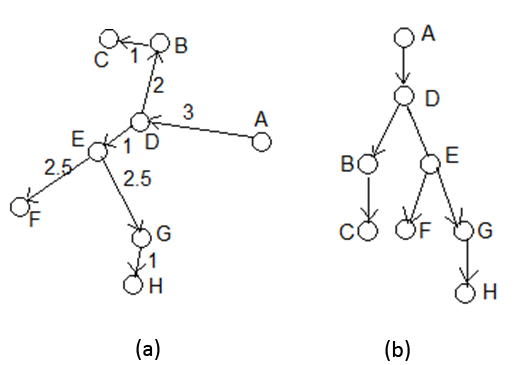
\includegraphics[scale=.5]{Figs/fig1.png}
  \caption{An example of FTP}
  \label{fig:example}
\end{figure}

\subsection{Applications}
One of the main applications of FTP is in distribution and transfer of data, and is considered when the sender and the receiver of the data should be physically near each other while transferring data. This proximity may be due to the security issues, or because of the cost of bandwidth in wireless communications. However, it can be used for distributing any other duplicatable commodities. FTP has also applications in broadcasting, routing, scheduling and network design~\cite{Arkin2006}.

\subsection{Related Work}
As mentioned before, Arkin, Bender, Fekete, Mitchell and Skutella~\cite{Arkin2006} have shown that in general, FTP is an NP-Hard problem. In another work, Arkin, Bender, Ge, He and Mitchell~\cite{Arkin2003} showed that even the FTP in unweighted graphs is NP-hard. They gave an ${ O(1)- }$approximation algorithm for the FTP in unweighted graphs.\\
In subsequent work on the FTP, Arkin, Bender, Fekete, Mitchell and Skutella~\cite{Arkin2006} Introduced a  ${ (1+\epsilon)- }$approximation algorithm (PTAS) for the geometric FTP in any fixed dimensions, which runs in
${ O(2^{O((1/\epsilon)^2 log⁡(1/\epsilon))}+n\log n) }$
time. They also gave an ${ O(1)- }$approximation algorithm which runs in ${ O(n\log n) }$ time. (This algorithm will be discussed later.)\\
Sztainberg, Arkin, Bender, and Mitchell~\cite{sztainberg2004} have studied heuristics for the FTP. They have shown that the greedy strategy gives ${ \Theta({\log n~}^{1-1/d}) }$ approximation bound, for the case that points are in a d-dimensional space. \\
More recently, Bucantanschi, Hoffmann, Hutson and Kretchmar~\cite{Bucantanschi2007} proposed another heuristic called ``Neighborhood Search Technique'' for the  FTP.\\
Könemann, Levin, and Sinha~\cite{Konemann2004} introduced an approximation algorithm for the general FTP which has an ${ O(\sqrt{\log n}) }$ approximation factor.

\subsection{Geometric Freeze-Tag Problem}
One of the variants of FTP, called the Geometric FTP, is which the robots are in a geometric (Euclidian) plane, and the distance between robots is the length of line segment connecting them. The geometric FTP is considered an open problem, and is listed as Problem \#35 on the well-known list ``The Open Problems Project''~\cite{OpenProblems}. However there are some approximation algorithms proposed to solve it.\\
In this paper, two approximation algorithms for the geometric FTP are discussed. In section 2 an approximation algorithm, introduced by Arkin et al.~\cite{Arkin2006} is discussed. In section 3 another algorithm with linear running time and a better approximation factor is introduced. And we wrap the paper up by concluding remarks in section 4.


\section{An Approximation Algorithm for the Geometric FTP}
In this section, an approximation algorithm is discussed for the geometric FTP. Its approximation factor is ${ O(1) }$, and its time complexity is ${ O(n\log n) }$, and it is proposed by Arkin, Bender, Fekete, Mitchell and Skutella [2]. This algorithm generates a wakeup tree whose makespan is ${ O(Radius(R)) }$, where $R$ is the set point of positions of robots, and ${ Radius(R) }$ is the radius of this set respect to the first awake robot. I.e. ${ Radius(R) }$ is the maximum distance of the first awake robot to any other member of $R$.\\
In this paper, it is assumed that the robots are located in a plane, and the speed of all the robots is constant and equals to one unit of speed, so that a robot requires $l$ units of time to travel $l$ units of distance.

\subsection{Describing the Algorithm}
For each point ${ v \in R }$, we partition the plane into $K$ sectors by rays emanating from $v$ at angles of
${ 0, ~2\pi/K, ~2(2\pi/K), ..., ~(K-1)(2\pi/K) }$
radians. We define $u_j(v)$ as the nearest point in the jth sector. (If there is no point of R in the jth sector, $u_j(v)$ is undefined.) All the $u_j(v)$ points can be found for every ${ v \in R }$ in ${ O(Kn\log n) }$ time with methods based on the standard Voronoi diagrams~\cite{Clarkson1987}.\\
Then, for each ${ v \in R }$, the points $u_j(v)$ are sorted in ascending order of their distance to $v$. Assume that for $v$, these points are sorted as ${ u_1,~u_2,...,~u_K }$. The awaking strategy is as follows: when the $v$ robot wakes up, it travels the path ${ <v,~u_1,~u_2,...,~u_K> }$, and wakes up the nearest robot in each non-empty sector surrounding it (Figure \ref{fig:thetagraph}). If any robot has been woken up before $v$ reaches it, $v$ skips awaking it.
\begin{figure} [h]
  \centering
  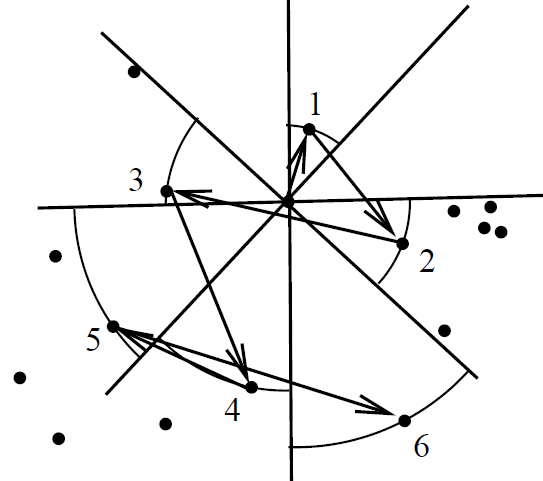
\includegraphics[scale=.5]{Figs/fig2.png}
  \caption{When $v$ is awakened, it wakes up each of the nearest robots in the $K$ sectors surrounding it, in order of increasing distance from $v$~\cite{Arkin2006}.}
  \label{fig:thetagraph}
\end{figure}

\subsection{The Performance of the Algorithm}
Here we discuss the performance of aforementioned algorithm. Assume ${ G_K=(R,E_K) }$ is a graph that connects each $v$ point to the $u_j(v)$ points that are the nearest neighbors in the $K$ sectors surrounding it. Hence, $G_K$ is a 
``$\theta-$graph'' for ${ \theta=2\pi/K }$ and if ${ K\geq 9 }$, it is a ``$t_\theta-$spanner'' for
${ t_\theta=1/(\cos\theta-\sin\theta) }$~\cite{Keil1992}.
This means that the graph distance of any two nodes of the graph $G_K$ for ${ K\geq 9 }$, is not greater than
{\small${ \dfrac{1}{\cos(2\pi/K)-\sin(2\pi/K)} }$}
times of the Euclidean distance of those two nodes. \\
Assume the first robot is in the point $v_0$ and the last robot that is woken up by this algorithm is in the point $v_l$. How much time is required to wake up $v_l$? We know that if the robot $v$ is woken up at time $t$, any $u_j$ neighbors of $v$ in the graph $G_K$ is reached in a time shorter than or equal to ${ t+\xi }$, where $\xi$ is the length of the path ${ <v,~u_1,~u_2,...,~u_K> }$. Let denote Euclidean distance and graph distance of $u$ and $v$ by ${ d(u,v) }$ and ${ d_{G_K}(u,v) }$ respectively. With a simple induction and the triangle inequality, it is concluded that:
{\small$$ \xi \leq (2j-1).d(v,u_j ) \leq (2K-1).d(v,u_j ) $$}
Thus $v_l$ is reached in a time that is no longer than ${ (2K-1) }$ times of the graph distance of $v_0$ and $v_l$ i.e. ${ d_{G_K}(v_0,v_l) }$, and because the graph is a ``$t_\theta-$spanner'' graph for ${ K\geq 9 }$, ${ d_{G_K}(v_0,v_l) }$ is not greater than
{\small${ \dfrac{d(v_0,v_l)}{\cos(2\pi/K)-\sin(2\pi/K)} }$}.
Therefore:\\
{\small\begin{align}
makespan(R)	&\leq (2K-1)~d_{G_K}(v_0,v_l) \nonumber\\
			&\leq \frac{2K-1}{\cos(2\pi/K)-\sin(2\pi/K)}~d(v_0,v_l) \nonumber
\end{align}}
\\
So, $v_l$ is woken up within the time of ${ O(d(v_0,v_l)) }$, and since ${ d(v_0,v_l) }$ is a lower bound for the optimum makespan, this algorithm is an ${ O(1)- }$approximation. \\
The time complexity of the algorithm is ${ O(n\log n) }$ for a constant $K$. We refer the reader to~\cite{Arkin2006} for more details.

\subsection{The Disadvantages of the Algorithm}
The aforementioned algorithm guarantees a constant approximation factor, but how high can this factor be? The upper bound of this factor is the function
{\small${ \dfrac{2K-1}{\cos(2\pi/K)-\sin(2\pi/K)} }$}
for ${ K\geq 9 }$. As seen on Figure \ref{fig:function}, this bound is greater than 57. In fact, the algorithm does not guarantee any approximation factors lower than 57.\\
Another disadvantage of this algorithm is its running time. Even though ${ O(n\log n) }$ suggests a rather good time complexity, but it does not seem to be optimal.
\begin{figure}[h]
  \centering
  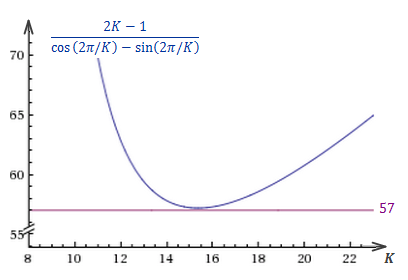
\includegraphics[scale=.5]{Figs/fig3.png}
  \caption{The function {\small${ \dfrac{2K-1}{\cos(2\pi/K)-\sin(2\pi/K)} }$} }
  \label{fig:function}
\end{figure}


\section{Proposed Algorithm for the Geometric FTP}
In this section, an approximation algorithm is introduced which has a constant approximation factor and runs in linear time. The advantage of this algorithm, compared to the previous algorithm, is its better running time and its lower approximation factor. The main idea is to split the area, in which the robots are, and to solve the problem in a divide and conquer manner by matching asleep robots to awake ones.\\
Assume there is one awake robot named $r$, and there are $n$ asleep robots; $R$ is a set of points corresponding to the asleep robots (Note that in this section, $R$ does not include the awake robot $r$.); ${ d=Diam(R) }$ is the diameter of $R$, which is the longest Euclidean distance between any two asleep robots; and $d_r$ is the radius of $R$ respect to $r$, which is the maximum Euclidean distance from $r$ to any member of $R$.\\
If so, an ${a\times b-}$rectangle with ${ a,b \leq d }$ can be found that encompasses all of the points of $R$, while its sides are parallel to the axes. If ${ r_1=(x_{min},y_1) }$ and ${ r_2=(x_{max},y_2) }$ are the points with the lowest and the highest $x$ values respectively, and ${ r_3=(x_3,y_{min}) }$ and ${ r_4=(x_4,y_{max}) }$ are the points with the lowest and the highest $y$ values respectively,
${ A=Rect \big( (x_{min},y_{min}),(x_{max},y_{max}) \big) }$
will be such rectangle as it is shown in the Figure~\ref{fig:split A}. \\
Now we find ${ m=(x_{med},y_{med})\in R }$, that is the median of $R$ in the lexicographical order based on $x$ and then $y$. (Which means if the points of $R$ are sorted in order of their $x$ values, and points with equal $x$ value are sorted in order of their $y$ values, $m$ will be the ${ \lceil\frac{n}{2}\rceil }$th point.) A hypothetical vertical line that passes through m splits the rectangle $A$ into two sections. At least one of these sections has the length of ${ a' \leq d/2 }$. We denote it by $A'$ and denote by $R'$, the points of $R$ which are located in $A'$, excluding the m point (Figure \ref{fig:split A}). In more precise terms:
{\small\begin{align}
&\mbox{if \ } x_{med}-x_{min} \leq \frac{d}{2}: \nonumber\\
&A'=Rect\big( (x'_{min}=x_{min},y_{min} ),(x'_{max}=x_{med},y_{max} )  \big) \nonumber\\
&R'=\big\{(x,y)\in R\ \big|\ x<x_{med} \mbox{ or } (x=x_{med} \mbox{ and } y<y_{med} )  \big\} \nonumber\\
\nonumber\\
&\mbox{if \ } x_{med}-x_{min}>\frac{d}{2}\ \ \ (\mbox{thus \ } x_{max}-x_{med}<\frac{d}{2}): \nonumber\\
&A'=Rect\big( (x'_{min}=x_{med},y_{min} ),( x'_{max}=x_{max},y_{max} )  \big) \nonumber\\
&R'=\big\{(x,y)\in R\ \big|\ x>x_{med} \mbox{ or } (x=x_{med} \mbox{ and } y>y_{med} ) \big\} \nonumber
\end{align}}
It is obvious that $R'$ has ${ \lceil\frac{n}{2}\rceil-1 }$ points and is encompassed by $A'$ which is an ${ a' \times b'- }$rectangle with ${ a' \leq \dfrac{d}{2} ,\ b'\leq d }$.
\begin{figure} [h]
  \centering
  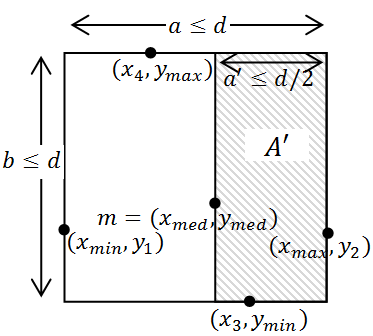
\includegraphics[scale=.5]{Figs/fig4.png}
  \caption{Splitting the rectangle $A$ vertically}
  \label{fig:split A}
\end{figure}\\
Now we find ${ m'=( x'_{med}, y'_{med})\in R' }$, which is the median of $R'$ in the lexicographical order based on $y$ and then $x$. Like the previous phase, a hypothetical horizontal line that passes through $m'$ divides $A'$ into two sections, and at least one of these sections will have the width of ${ b'' \leq d/2 }$. We denote it by $A''$ and denote by $R''$, the points of $R$ which are located in $A''$, excluding the $m$ point (Figure \ref{fig:split A'}). In more precise terms:
{\small\begin{align}
&\mbox{if \ } y'_{med}-y_{min} \leq \frac{d}{2}: \nonumber\\
&A''=Rect\big( (x'_{min},y_{min} ),(x'_{max},y'_{med} )  \big) \nonumber\\
&R''=\big\{(x,y)\in R'\ \big|\ y<y'_{med} \mbox{ or } (y=y'_{med} \mbox{ and } x<x'_{med} )  \big\} \nonumber\\
\nonumber\\
&\mbox{if \ } y'_{med}-y_{min}>\frac{d}{2}\ \ \ (\mbox{thus \ } y_{max}-y'_{med}<\frac{d}{2}): \nonumber\\
&A''=Rect\big( (x'_{min},y'_{med} ),( x'_{max},y_{max} )  \big) \nonumber\\
&R''=\big\{(x,y)\in R'\ \big|\ y>y'_{med} \mbox{ or } (y=y'_{med} \mbox{ and } x>x'_{med} ) \big\} \nonumber
\end{align}}
It is obvious that $R''$ has ${ \big\lceil\dfrac{|R'|}{2}\big\rceil < n/4 }$ points and is encompassed by an ${ a'' \times b''- }$rectangle (which is $A''$).
After this introduction now we are ready to describe the algorithm.
\begin{figure} [h]
  \centering
  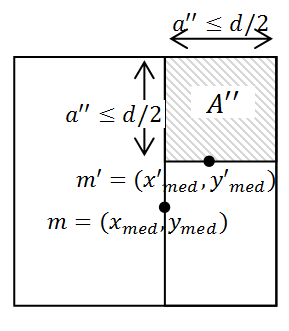
\includegraphics[scale=.5]{Figs/fig5.png}
  \caption{Splitting the rectangle $A'$ horizontally}
  \label{fig:split A'}
\end{figure}

\subsection{Describing the Algorithm}
We call this algorithm \textit{ApproxFTP} algorithm hereafter. \textit{ApproxFTP}  inputs $r$ as the only awake robot and $R$ as the set of the asleep robots, and provides an awaking schedule.\\
If ${|R| \leq 3 }$, $r$ wakes up an asleep robot. This is done in a time not more than $d_r$.  So there will be at most two asleep robots remaining, which can be woken up by the two awake robots working in parallel. This is done in a time not more than ${ \sqrt{2}~d }$. (Since the robots are in a rectangle which its length and width are at most $d$, the distance between any two robots is not greater than ${ \sqrt{2}~d }$.) Therefore the whole awakening process can be done in a time not more than ${ d_r+\sqrt{2}~d }$.\\
For ${|R| \geq 4 }$, the algorithm works recursively. First, it finds the $A'$ and $A''$ rectangles and the $R'$ and $R''$ sets as it was described before. Then the algorithm runs with $r$ and $R''$ as inputs to awake all the robots of $R''$. Notice that the awake robots are not necessarily in their initial places, but they are definitely in places where some robots of $R''$ were initially there. Thus, all the awaken robots, including $r$, are located in $A''$.\\
Now, the number of the asleep robots remaining in $R'$ is less than or equal to the number of the awake robots, which are the members of  ${ R'' \cup \{r\} }$:
{\small$$ |R'-R''|=|R'|-(\bigg\lceil\frac{|R'|}{2}\bigg\rceil-1) \leq \bigg\lceil\frac{|R'|}{2}\bigg\rceil = |R''|+1 $$}
So, we assign to any robot of ${ R'-R'' }$, one of the robots of ${ R'' \cup \{r\} }$. This assignment constructs a maximum matching between ${ R'-R'' }$ and ${ R'' \cup \{r\} }$. To wake up all the robots of $R'$, each of the asleep robots of ${ R'-R'' }$ can be awakened by its assigned robot of ${ R'' \cup \{r\} }$. Since the robots work in parallel, the time needed for this phase is at most equal to the diagonal of $A'$ which is not more than ${ \sqrt{5}/2~d }$.\\
After this phase, $r$ and all the robots of $R'$ are awake and all of them are located in $A'$. Here again since the number of robots of ${ R-R' }$ is not more than the number of the awake robots ${ R' \cup \{r\} }$, they can be awaken in parallel in one phase. And the time needed to do this is at most equal to the diagonal of $A$ which is not more than ${\sqrt{2}~d }$.

\subsection{The Approximation Factor of ApproxFTP}
In this section, we assess the approximation factor of the proposed algorithm.

\begin{lemma}
\label{lem:1}
The time needed to wake up $n$ asleep robots which are located inside a rectangle with its sides parallel to the axes, and has a length and width shorter than or equal to $d$, by a robot whose distance from the asleep robots is at most $d_r$, with \textit{ApproxFTP} will not be more than ${ (2\sqrt{2}+\sqrt{5})d+d_r }$.
\end{lemma}
\begin{proof}
If ${ makespan(n,d) }$ is the required time to wake up $n$ robots with the aforementioned conditions, as it was stated in Describing the Algorithm part, for ${ n\geq 4 }$ we have:
{\small\begin{align}
makespan(n,d) &\leq makespan(\bigg\lceil \frac{\lceil\frac{n}{2}\rceil\!\!-\!1}{2} \bigg\rceil\!\!-\!1, \frac{d}{2})+\!\sqrt{2}d+\!\frac{\sqrt{5}}{2}d \nonumber\\
				&\leq makespan(\frac{n}{4}, \frac{d}{2})+(\sqrt{2}+\frac{\sqrt{5}}{2})d \nonumber
\end{align}}
and for ${ n\le 4 }$:
{\small$$ makespan(n,d) \leq \sqrt{2} ~d+d_r $$}
By solving this recursive relation we have:
{\small\begin{align}
makespan(n,d) &\leq (2\sqrt{2}+\!\sqrt{5})d-\!(\sqrt{2}+\!\frac{\sqrt{5}}{2}) 2^{-\!\lfloor\log_4n \rfloor}+d_r \nonumber\\
				&\leq (2\sqrt{2}+\!\sqrt{5})d+d_r \nonumber
\end{align}}
\end{proof}

It is worth mentioning that in the first call of the algorithm, in which ${ d=Diam(R) }$, the distance between each pair of robots is less than or equal to $d$, while in the next calls the distance of two robots can be as long as the diagonal of the encompassing rectangle. This is the same distance that has appeared as ${ \sqrt{5}/2~d }$ and ${ \sqrt{2}~d }$ in our computations. But only for the first call, we can be assured that the distance of the robots is at most $d$, instead of  ${ \sqrt{5}/2~d }$ and ${ \sqrt{2}~d }$. The following lemma uses this.

\begin{lemma}
\label{lem:2}
The time required to wake up $n$ robots, corresponding to points in the $R$ set, with one awake robot in the beginning whose distance from the points of $R$ is at most $d_r$, using \textit{ApproxFTP} algorithm, is not shorter than or equal to
${ (2+\sqrt{2}+\sqrt{5}/2)Diam(R)+d_r }$.
\end{lemma}
\begin{proof}
In the first call of the algorithm, the distance of the robots from each other is at most ${ Diam(R) }$, so after awaking all the robots of $R''$, the other robots of $R$ can be woken up in two phases, each of which require a time not more than ${ Diam(R) }$. Hence:
{\small$$ makespan(R) \leq makespan(\frac{n}{4},\frac{Diam(R)}{2})+2Diam(R) $$}
For next calls of the algorithm, we use Lemma \ref{lem:1}:
{\small$$ makespan(\frac{n}{4},\frac{Diam(R)}{2}) \leq (2\sqrt{2}+\!\sqrt{5})\frac{Diam(R)}{2}+d_r $$}
and as a result:
{\small\begin{align}
makespan(R) &\leq (2\sqrt{2}+\!\sqrt{5})\frac{Diam(R)}{2}+d_r+2 Diam(R) \nonumber\\
			&\leq (2+\sqrt{2}+\frac{\sqrt{5}}{2})Diam(R)+d_r \nonumber
\end{align}}
\end{proof}

\begin{theorem}
ApproxFTP has an approximation factor which is at most $10.1$.
\end{theorem}
\begin{proof}
In the previous lemma it was proven that:
{\small$$ makespan(R) \leq (2+\sqrt{2}+\frac{\sqrt{5}}{2})Diam(R)+d_r $$}
We know that ${ Diam(R) \leq 2d_r }$, because if we draw a circle with $r$ as the center and $d_r$ as the radius, it will encompass all of the points in $R$ and the distance of any two points in this circle is less than or equal to its diameter. Hence:
{\small$$ makespan(R) \leq (5+2\sqrt{2}+\sqrt{5})d_r \leq 10.1~d_r $$}
Since $d_r$ is a lower bound for the optimum makespan, \textit{ApproxFTP} is an approximation algorithm with a constant approximation factor which is at most $10.1$.
\end{proof}

\subsection{The Time Complexity of ApproxFTP}
To compute the time complexity of this algorithm, it should be noted that finding the median of a set with $n$ members is possible in $O(n)$ time~\cite{CLRS}. So, the algorithm can find $A'$, $A''$, $R'$ and $R''$ in $O(n)$ time. Then, the algorithm is called with $R''$ as its input. The number of the members of $R''$ is less than $n/4$. After that, the algorithm finds matchings between the members of ${ R'-R'' }$ and ${ R''\cup\{r\} }$, and the members of ${ R-R' }$ and ${ R'\cup\{r\} }$. This phases can also be done in $O(n)$.\\
So, if the running time of algorithm for ${ |R|=n }$ is shown as $T(n)$,
{\small\begin{align}
T(n)&=T(\frac{n}{4})+O(n) &n\geq 4 \nonumber\\
T(n)&=O(1) &n\leq 3 \nonumber
\end{align}}
By solving this recursive relation, we find out that ${ T(n)=O(n) }$; so the \textit{ApproxFTP}  runs in linear time.


\section{Conclusion}
In this paper, we studied the Freeze-Tag Problem, which is NP-Hard in general, and its geometric variant is an open. Then, a constant factor approximation algorithm for the geometric Freeze-Tag Problem was introduced, which outperforms the previous constant factor approximation algorithm of Akin et al.~\cite{Arkin2006} in terms of running time and approximation factor.


%---------------------------- Bibliography -------------------------------

% Please add the contents of the .bbl file that you generate,  or add bibitem entries manually if you like.
% The entries should be in alphabetical order
\small
\bibliographystyle{abbrv}
\bibliography{References}


\end{document}
